\chapter{Appendix}
This appendix presents the open-source contribution and the Sustainable Development Goals associated with the project.

\section{Open Source Contribution}
\begin{itemize}[nosep]
\item \textbf{Project / Repository:} Lastbook
\item \textbf{Platform:} GitHub
\item \textbf{Student contributors:} Rushikesh Tathe, Nihar Gudekar, and Mohammad Ali Sayyed
\item \textbf{Nature of contribution:} Added a video playback-speed selector with options from 0.5$\times$ to 2$\times$, synchronised with the video. The change was tested in Microsoft Edge and with the project test suite.
\item \textbf{Pull request:} \#132, submitted and awaiting review.
\item \textbf{Repository:} \textcolor{blue}{\url{https://github.com/Immortal-Protocols/lastbook}}
\item \textbf{Pull request link:} \textcolor{blue}{\url{https://github.com/Immortal-Protocols/lastbook/pull/132}}
\end{itemize}
\subsection{Evidence}
The following screenshots show the contribution branch and its commit history.
\begin{figure}[H]
\centering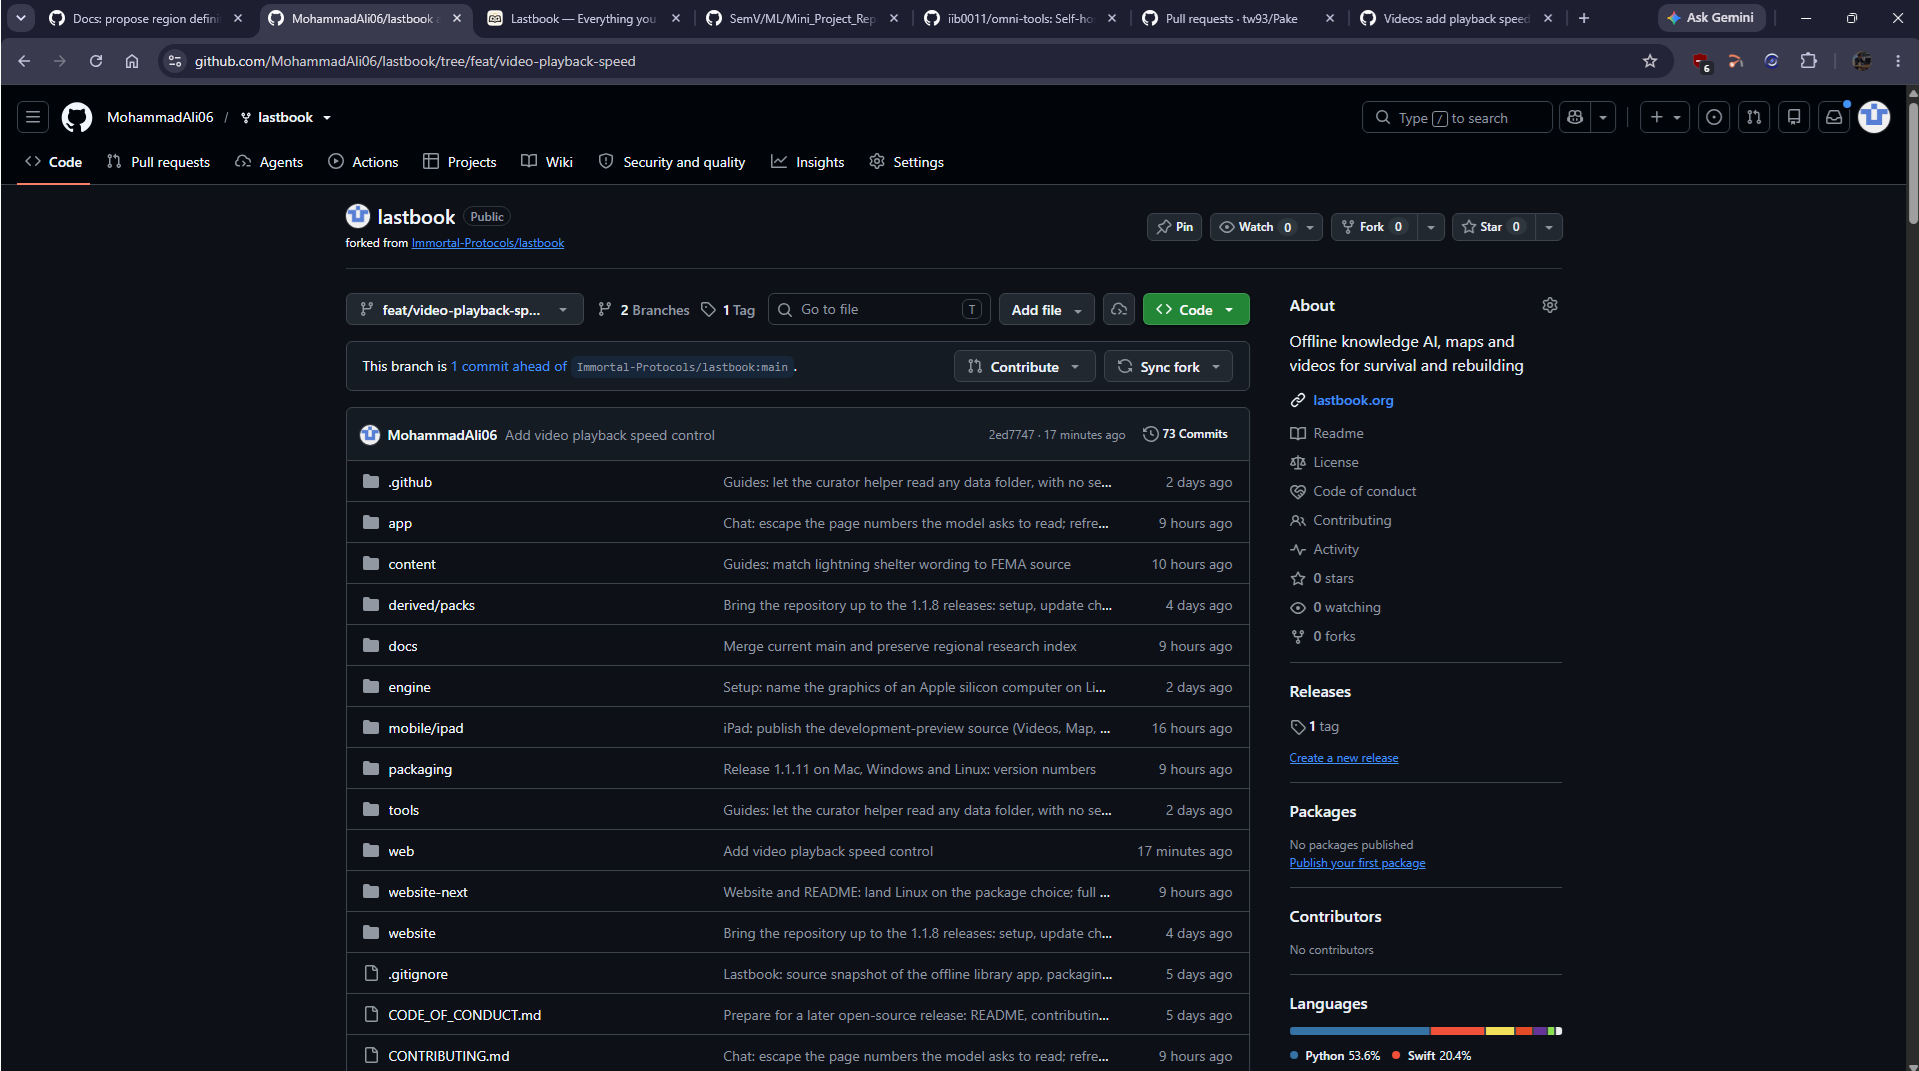
\includegraphics[width=0.96\textwidth,height=0.37\textheight,keepaspectratio]{figures/lastbook_pr.png}
\caption{Lastbook playback-speed contribution branch}
\end{figure}
\begin{figure}[H]
\centering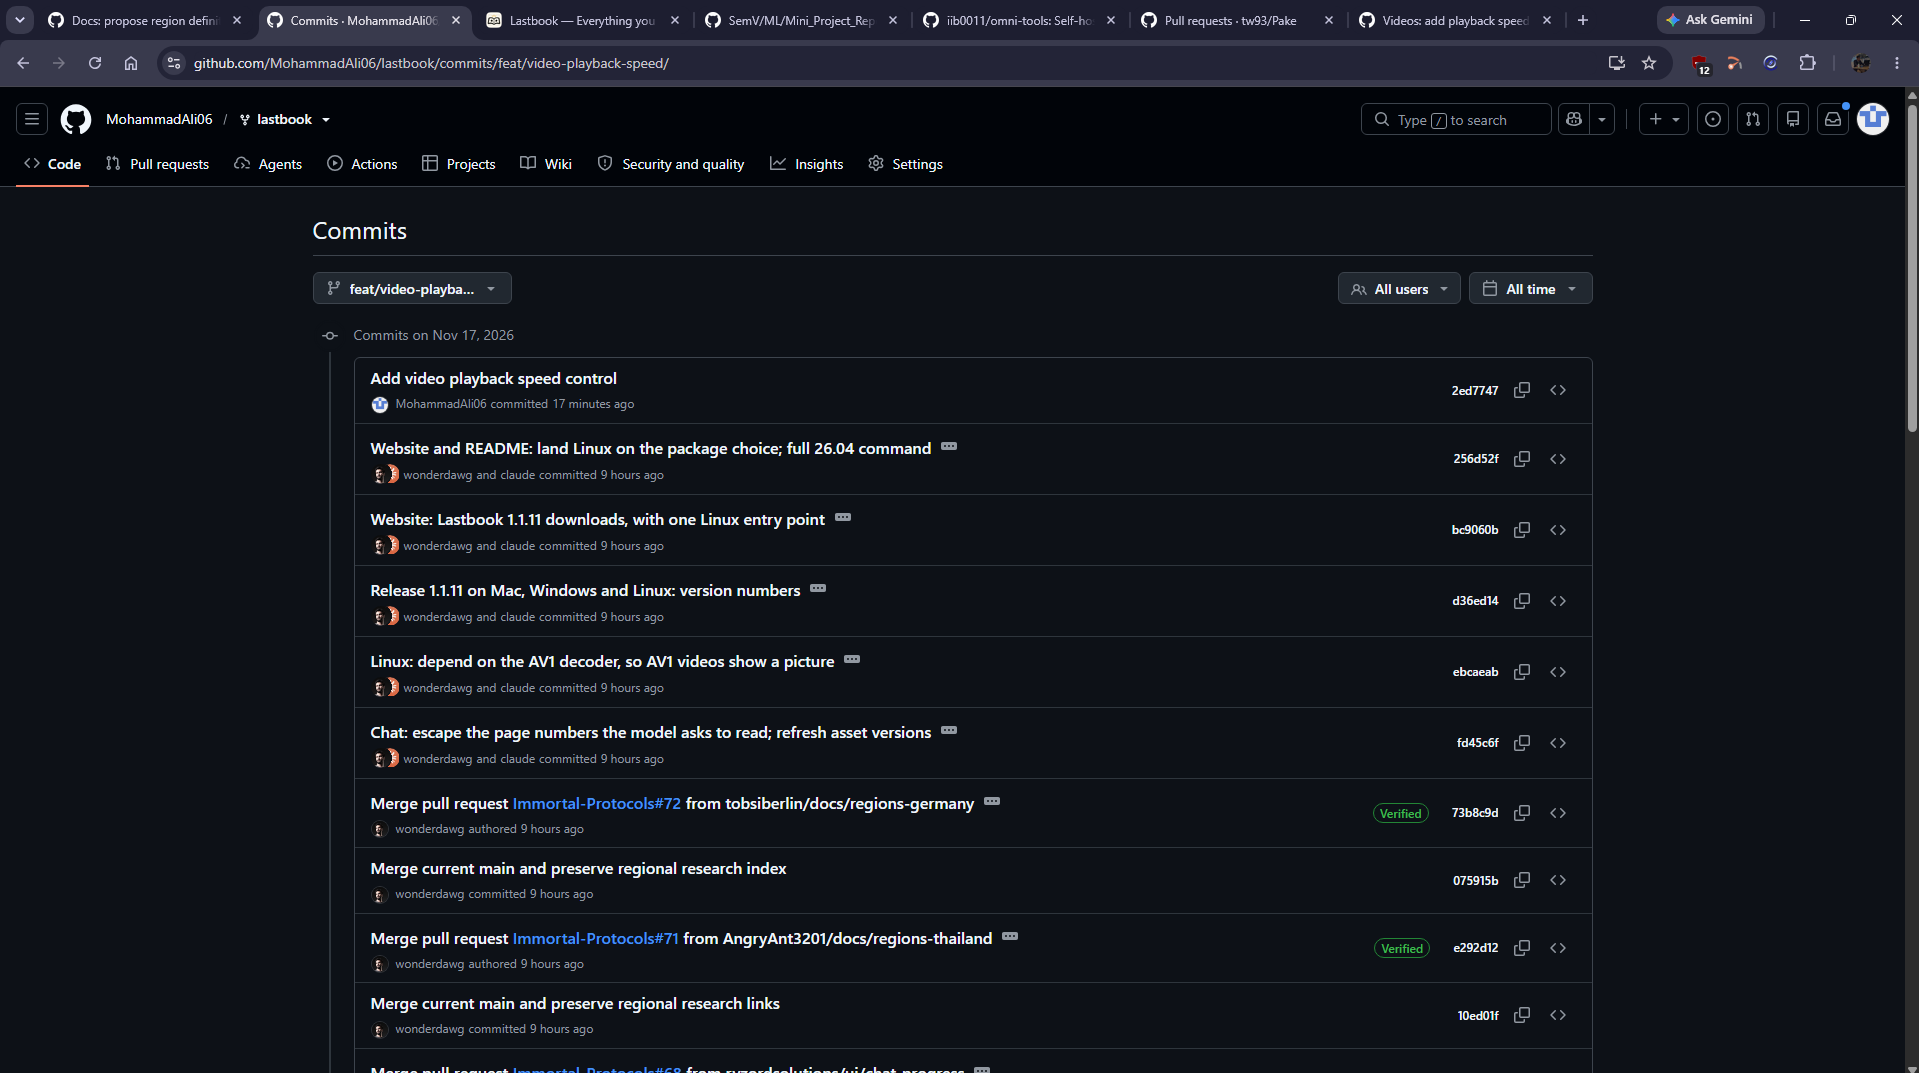
\includegraphics[width=0.96\textwidth,height=0.37\textheight,keepaspectratio]{figures/lastbook_commit.png}
\caption{Commit associated with the contribution}
\end{figure}
\section{SDG Goals Achieved}
The project and open-source contribution indirectly support the following goals:
\begin{itemize}
\item \textbf{SDG 3 -- Good Health and Well-being:} Analysing model robustness on a medical dataset encourages attention to data quality in health-related decision support.
\item \textbf{SDG 4 -- Quality Education:} The reproducible benchmark supports learning about data quality and machine-learning evaluation; adjustable playback speed can help viewers learn at their preferred pace.
\item \textbf{SDG 9 -- Industry, Innovation and Infrastructure:} Reproducible experiment tooling and the open-source software contribution support accessible, reusable digital infrastructure.
\end{itemize}

